%%%%%%%%%%%%%%%%%%%%%%%%%%%%%%%%%%%%%%%%%
% Beamer Presentation
% LaTeX Template
% Version 1.0 (10/11/12)
%
% This template has been downloaded from:
% http://www.LaTeXTemplates.com
%
% License:
% CC BY-NC-SA 3.0 (http://creativecommons.org/licenses/by-nc-sa/3.0/)
%
%%%%%%%%%%%%%%%%%%%%%%%%%%%%%%%%%%%%%%%%%

%----------------------------------------------------------------------------------------
%	PACKAGES AND THEMES
%----------------------------------------------------------------------------------------

\documentclass[10pt]{beamer}

\mode<presentation> {

% The Beamer class comes with a number of default slide themes
% which change the colors and layouts of slides. Below this is a list
% of all the themes, uncomment each in turn to see what they look like.

\renewcommand{\familydefault}{\rmdefault}

\graphicspath{ {./figures/} }
\usepackage{graphicx} % Allows including images
\usepackage{booktabs} % Allows the use of \toprule, \midrule and \bottomrule in tables
\usepackage{tikz} % Allows the use of \toprule, \midrule and \bottomrule in tables
\usepackage{hyperref}
\usepackage[printwatermark]{xwatermark}

\usetheme{default}
% \usetheme{AnnArbor}
% \usetheme{Antibes}
% \usetheme{Bergen}
% \usetheme{Berkeley}
% \usetheme{Berlin}
% \usetheme{Boadilla}
% \usetheme{CambridgeUS}
% \usetheme{Copenhagen}
% \usetheme{Darmstadt}
% \usetheme{Dresden}
% \usetheme{Frankfurt}
% \usetheme{Goettingen}
% \usetheme{Hannover}
% \usetheme{Ilmenau}
% \usetheme{JuanLesPins}
% \usetheme{Luebeck}
% \usetheme{Madrid}
% \usetheme{Malmoe}
% \usetheme{Marburg}
% \usetheme{Montpellier}
% \usetheme{PaloAlto}
% \usetheme{Pittsburgh}
% \usetheme{Rochester}
% \usetheme{Singapore}
% \usetheme{Szeged}
% \usetheme{Warsaw}

% As well as themes, the Beamer class has a number of color themes
% for any slide theme. Uncomment each of these in turn to see how it
% changes the colors of your current slide theme.

% \usecolortheme{albatross}
\usecolortheme{beaver}
% \usecolortheme{beetle}
% \usecolortheme{crane}
% \usecolortheme{dolphin}
% \usecolortheme{dove}
% \usecolortheme{fly}
% \usecolortheme{lily}
% \usecolortheme{orchid}
% \usecolortheme{rose}
% \usecolortheme{seagull}
% \usecolortheme{seahorse}
% \usecolortheme{whale}
% \usecolortheme{wolverine}

%\setbeamertemplate{footline} % To remove the footer line in all slides uncomment this line
% \setbeamertemplate{footline}[page number] % To replace the footer line in all slides with a simple slide count uncomment this line

\setbeamertemplate{navigation symbols}{} % To remove the navigation symbols from the bottom of all slides uncomment this line

% \setbeamertemplate{background}{
%     \tikz[overlay,remember picture]\node[opacity=0.4]at (current page.center){
%         \includegraphics[width=2cm]{iot_analytics_logo.jpg}
%         }}

}

%----------------------------------------------------------------------------------------
%	TITLE PAGE
%----------------------------------------------------------------------------------------

\title[Credit Default Prediction]{Proposed Analytic Framework} % The short title appears at the bottom of every slide, the full title is only on the title page

\author{Tuomo Kareoja} % Your name
\institute[Alert! Analytics] % Your institution as it will appear on the bottom of every slide, may be shorthand to save space
{
Alert! Analytics \\ % Your institution for the title page
\medskip
}
\date{\today} % Date, can be changed to a custom date

\begin{document}

\begin{frame}
\titlepage % Print the title page as the first slide
\end{frame}

% \begin{frame}
% \frametitle{Agenda} % Table of contents slide, comment this block out to remove it
% \tableofcontents % Throughout your presentation, if you choose to use \section{} and \subsection{} commands, these will automatically be printed on this slide as an overview of your presentation
% \end{frame}

%----------------------------------------------------------------------------------------
%	PRESENTATION SLIDES
%----------------------------------------------------------------------------------------

\begin{frame}
\frametitle{Analytic Process}

\bigskip
\bigskip
{
    \centering
    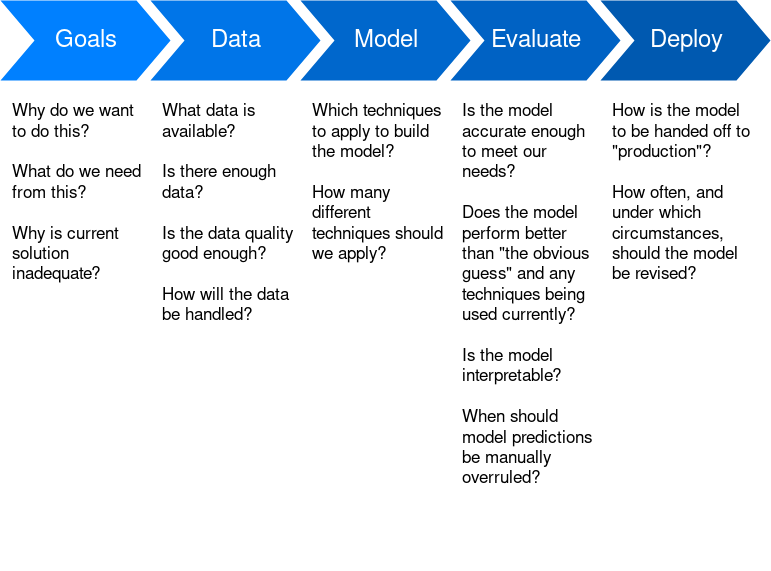
\includegraphics[width=\textwidth,height=\textheight,keepaspectratio]{analysis_flow.png}
    \par
}

\end{frame}


\begin{frame}
\frametitle{Goals}

\begin{itemize}
    \item Why do we want to do this?
    \pause
    \begin{itemize}
        \item Increasing number of customers who default
        \pause
        \item Risk of losing customers to other credit rating agencies
        if our predictions don't get better
        \pause
    \end{itemize}
    \item What do we need from this?
    \pause
    \begin{itemize}
        \item Better predictive model, so that less people who would default on
        their loans don't get loans or get only smaller loans
        \pause
    \end{itemize}
    \item Why is the current solution inadequate?
    \pause
    \begin{itemize}
        \item Too many will-be-defaulters get loans or the get loans that are too big
        \pause
        \item QUESTION? Why don't make the current model more stringent?
    \end{itemize}
\end{itemize}

\end{frame}


\begin{frame}
\frametitle{Data}

\begin{itemize}
    \item What data is available?
    \pause
    \begin{itemize}
        \item Information about 30000 customers payment default status with
        demographic information and 6 month of information about previous loan amounts
        and payments
        \pause
    \end{itemize}
    \item Is the data quality good enough?
    \pause
    \begin{itemize}
        \item Almost no missing data
        \pause
        \item Dataset information given does not match the data on all columns
        \pause
        \item Data is from 2005. Has there been no significant changes since then?
        \pause
    \end{itemize}
    \item Is there enough data?
    \pause
    \begin{itemize}
        \item about 20 \% of customers default in the data.
        Is this the true rate for all customers?
        \pause
        \item More data would mean more precise models.
        Even 10X current data size would be easily handled
        \pause
    \end{itemize}
    \item How will the data be handled?
    \pause
    \begin{itemize}
        \item Locally on one computer
        \pause
        \item Erased at the end of the project
    \end{itemize}
\end{itemize}

\end{frame}

\begin{frame}
\frametitle{The End}

\LARGE{\centerline{Questions?}}

\end{frame}

%----------------------------------------------------------------------------------------

\end{document}
